\title{COM S 352 Homework 2}
\author{Alec Meyer}

\date{\today}

\documentclass[11pt]{article}
\usepackage{changepage}
\usepackage{graphicx}
\usepackage{amsmath}
\graphicspath{ {./images/} }
\newcommand\tab[1][1cm]{\hspace*{#1}}
\usepackage{amssymb}


\begin{document}
\maketitle


\section*{Question 1}
    First, the kernel saves the context of the old process
    in its PCB and loads the saved data of the new process.
\section*{Question 2}
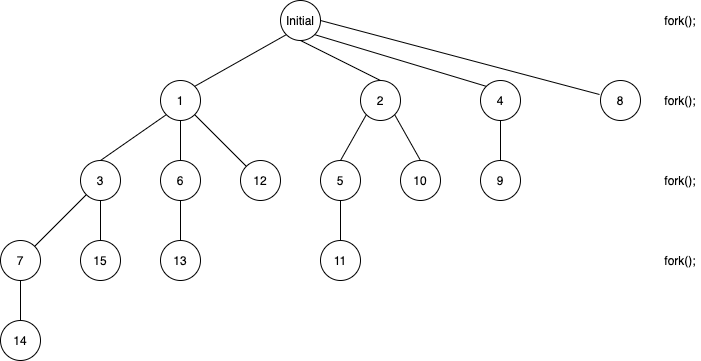
\includegraphics[scale=0.52]{COMS352HW2Q2}
16 processes

\section*{Question 3}

\section*{Question 4}
parent C: pid = 32259\\
parent D: pid1 = 32257\\
child A: pid = 0\\
child B: pid1 = 32259\\
\section*{Question 5}

\section*{Question 6}


\section*{Question 7}

\end{document}